\documentclass[12pt]{article}

\usepackage[a4paper,margin=2.5cm]{geometry}
\usepackage{amsmath, amssymb, amsthm}
\usepackage{bm}
\usepackage{hyperref}
\usepackage{graphicx}
\usepackage{caption}
\usepackage{listings}
\usepackage{xcolor}
\usepackage{float}
\usepackage{placeins}
\graphicspath{{figures/}}

\lstdefinestyle{code}{
  basicstyle=\ttfamily\small,
  numbers=left,
  numberstyle=\tiny,
  numbersep=8pt,
  keywordstyle=\color{blue},
  commentstyle=\color{teal!70!black},
  stringstyle=\color{orange!70!black},
  showstringspaces=false,
  breaklines=true,
  frame=single,
  framerule=0.3pt,
  rulecolor=\color{black!15}
}
\lstset{style=code}

\title{Local Outlier Factor Tutorial}
\author{}
\date{\today}

\begin{document}
\maketitle

\section{Introduction}
Local Outlier Factor (LOF) detects anomalies by comparing the local density of a point to that of its neighbors. Points with significantly lower density than their neighbors receive large LOF scores, signalling potential outliers. LOF excels at identifying anomalies in data with varying densities where global distance-based thresholds may fail.

\section{Theory and Formulas}
\subsection{$k$-Distance and Reachability}
For a point \(\mathbf{x}\) and neighborhood size \(k\), the \(k\)-distance \(d_k(\mathbf{x})\) is the distance to the \(k\)-th nearest neighbor. The reachability distance from \(\mathbf{x}\) to neighbor \(\mathbf{y}\) is defined as
\begin{equation}
\operatorname{reach}_k(\mathbf{x}, \mathbf{y}) = \max\{ d_k(\mathbf{y}), \lVert \mathbf{x} - \mathbf{y} \rVert_2 \}.
\end{equation}

\subsection{Local Reachability Density and LOF}
The local reachability density (LRD) of \(\mathbf{x}\) is the inverse of the average reachability distance to its neighborhood \(N_k(\mathbf{x})\):
\begin{equation}
\operatorname{lrd}_k(\mathbf{x}) = \left( \frac{1}{|N_k(\mathbf{x})|} \sum_{\mathbf{y} \in N_k(\mathbf{x})} \operatorname{reach}_k(\mathbf{x}, \mathbf{y}) \right)^{-1}.
\end{equation}
The LOF score compares \(\operatorname{lrd}_k\) at \(\mathbf{x}\) to the densities of its neighbors:
\begin{equation}
\operatorname{LOF}_k(\mathbf{x}) = \frac{1}{|N_k(\mathbf{x})|} \sum_{\mathbf{y} \in N_k(\mathbf{x})} \frac{\operatorname{lrd}_k(\mathbf{y})}{\operatorname{lrd}_k(\mathbf{x})}.
\end{equation}
Values near 1 indicate density comparable to neighbors, while scores significantly above 1 suggest anomalies.

\subsection{Hyperparameters and Practical Notes}
Choosing \(k\) controls the locality of the detector; small \(k\) may overreact to noise, whereas large \(k\) blurs local structure. Distance metrics, feature scaling, and handling of categorical variables also influence performance. LOF scores are relative, so a decision threshold must be selected based on application-specific tolerances or contamination estimates.

\section{Applications and Tips}
\begin{itemize}
  \item \textbf{Network intrusion detection}: surface unusual traffic patterns in high-dimensional log data.
  \item \textbf{Industrial monitoring}: detect sensor drifts or faults that reduce local density in feature space.
  \item \textbf{Fraud analytics}: identify customer behavior that deviates sharply from peer groups.
  \item \textbf{Best practices}: standardize features, experiment with multiple \(k\) values, inspect LOF score distributions, and combine with domain knowledge to validate flagged points.
\end{itemize}

\section{Python Practice}
The script \texttt{gen\_lof\_figures.py} synthesizes a dataset with dense clusters and scattered anomalies, fits scikit-learn's \texttt{LocalOutlierFactor}, and exports a score heatmap and histogram illustrating the separation between inliers and outliers.
\begin{lstlisting}[language=Python,caption={Excerpt from gen_lof_figures.py}]
from sklearn.neighbors import LocalOutlierFactor

lof = LocalOutlierFactor(n_neighbors=35, contamination=0.08)
pred = lof.fit_predict(points)
scores = -lof.negative_outlier_factor_
\end{lstlisting}

\section{Result}
\begin{figure}[H]
  \centering
  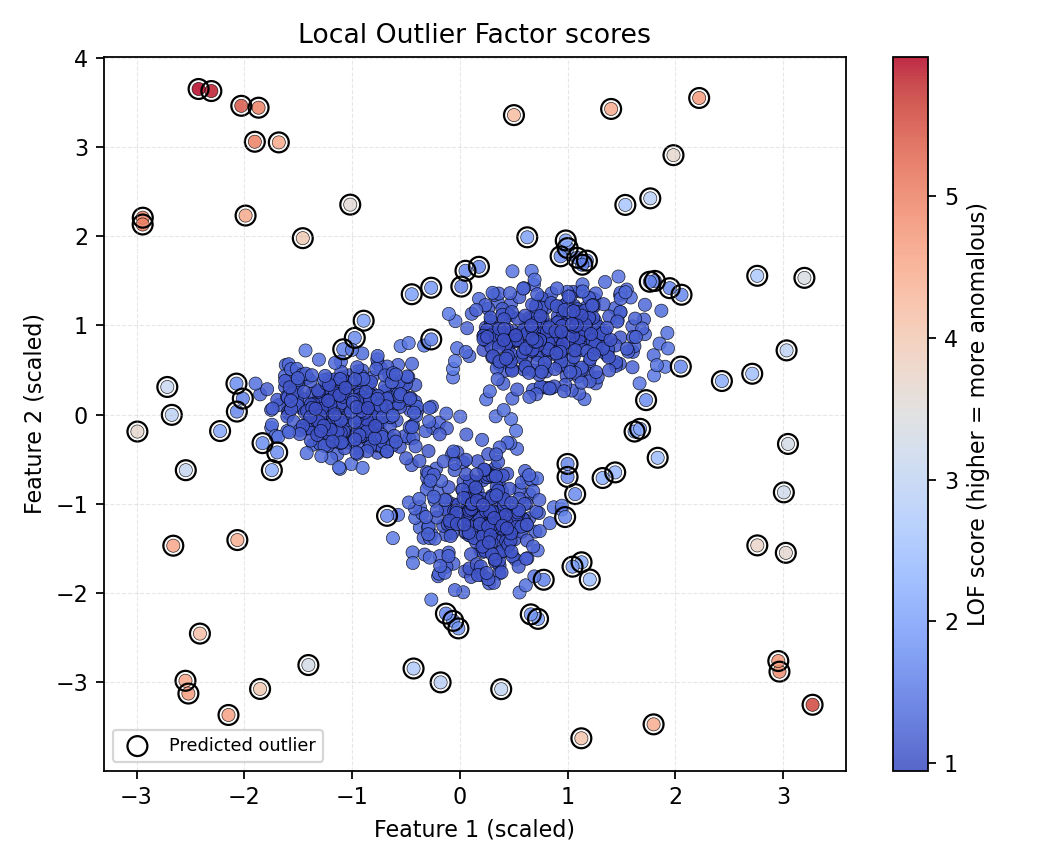
\includegraphics[width=0.82\linewidth]{lof_decision_map.png}
  \caption{LOF scores across the feature space; higher scores highlight sparser regions}
  \label{fig:lof_decision_map}
\end{figure}

\begin{figure}[H]
  \centering
  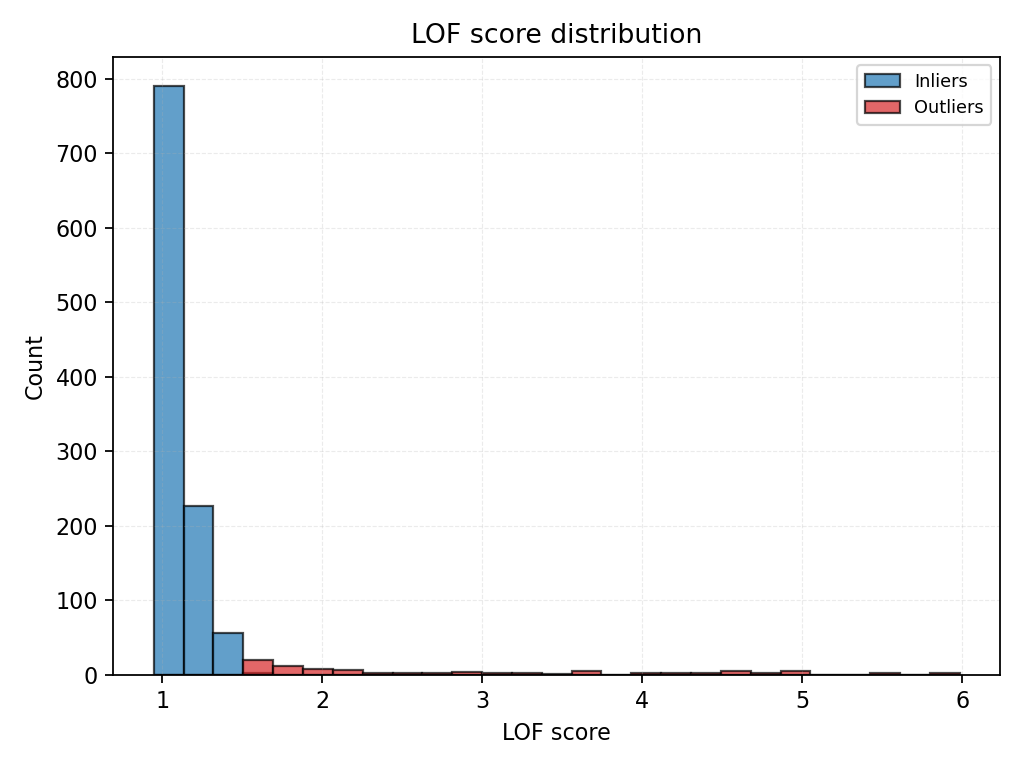
\includegraphics[width=0.78\linewidth]{lof_score_hist.png}
  \caption{Histogram of LOF scores comparing predicted inliers and outliers}
  \label{fig:lof_score_hist}
\end{figure}

\FloatBarrier
\section{Summary}
LOF evaluates relative local density to flag anomalies, making it effective on data with heterogeneous cluster structure. Proper scaling, neighborhood tuning, and score visualization enable robust deployments in security, industrial, and financial monitoring. The synthetic example demonstrates how LOF separates sparse points from dense clusters and how score distributions guide threshold selection.

\end{document}